\section{Vincoli}
\subsection{Vincoli tecnologici}\label{chap:vincoli tec}

{\company} non impone vincoli specifici sulle tecnologie da utilizzare. Tuttavia, essendo lo scopo del progetto lo 
sviluppo di un modulo per un'applicazione esistente, emergono vincoli tecnologici impliciti. È necessario utilizzare gli 
stessi \textit{framework} già impiegati per lo sviluppo, per poter integrare il modulo nell'\textit{app} ed eventualmente 
riportarlo nel \textit{software} commercializzato.\\
Non vi sono divieti circa l'introduzione di nuove tecnologie. Come riporto nel capitolo \ref{chap:strategia}, uno degli obiettivi
aziendali per il progetto di \textit{stage} è valutare il beneficio di nuove librerie, \textit{framework}
e tecnologie per favorire innovazione e crescita.\\
Anche per gli strumenti da utilizzare non ho ricevuto vincoli espliciti, eccetto l'uso di BitBucket
come piattaforma per conservare il codice.

\begin{figure}[H]
      \centering
      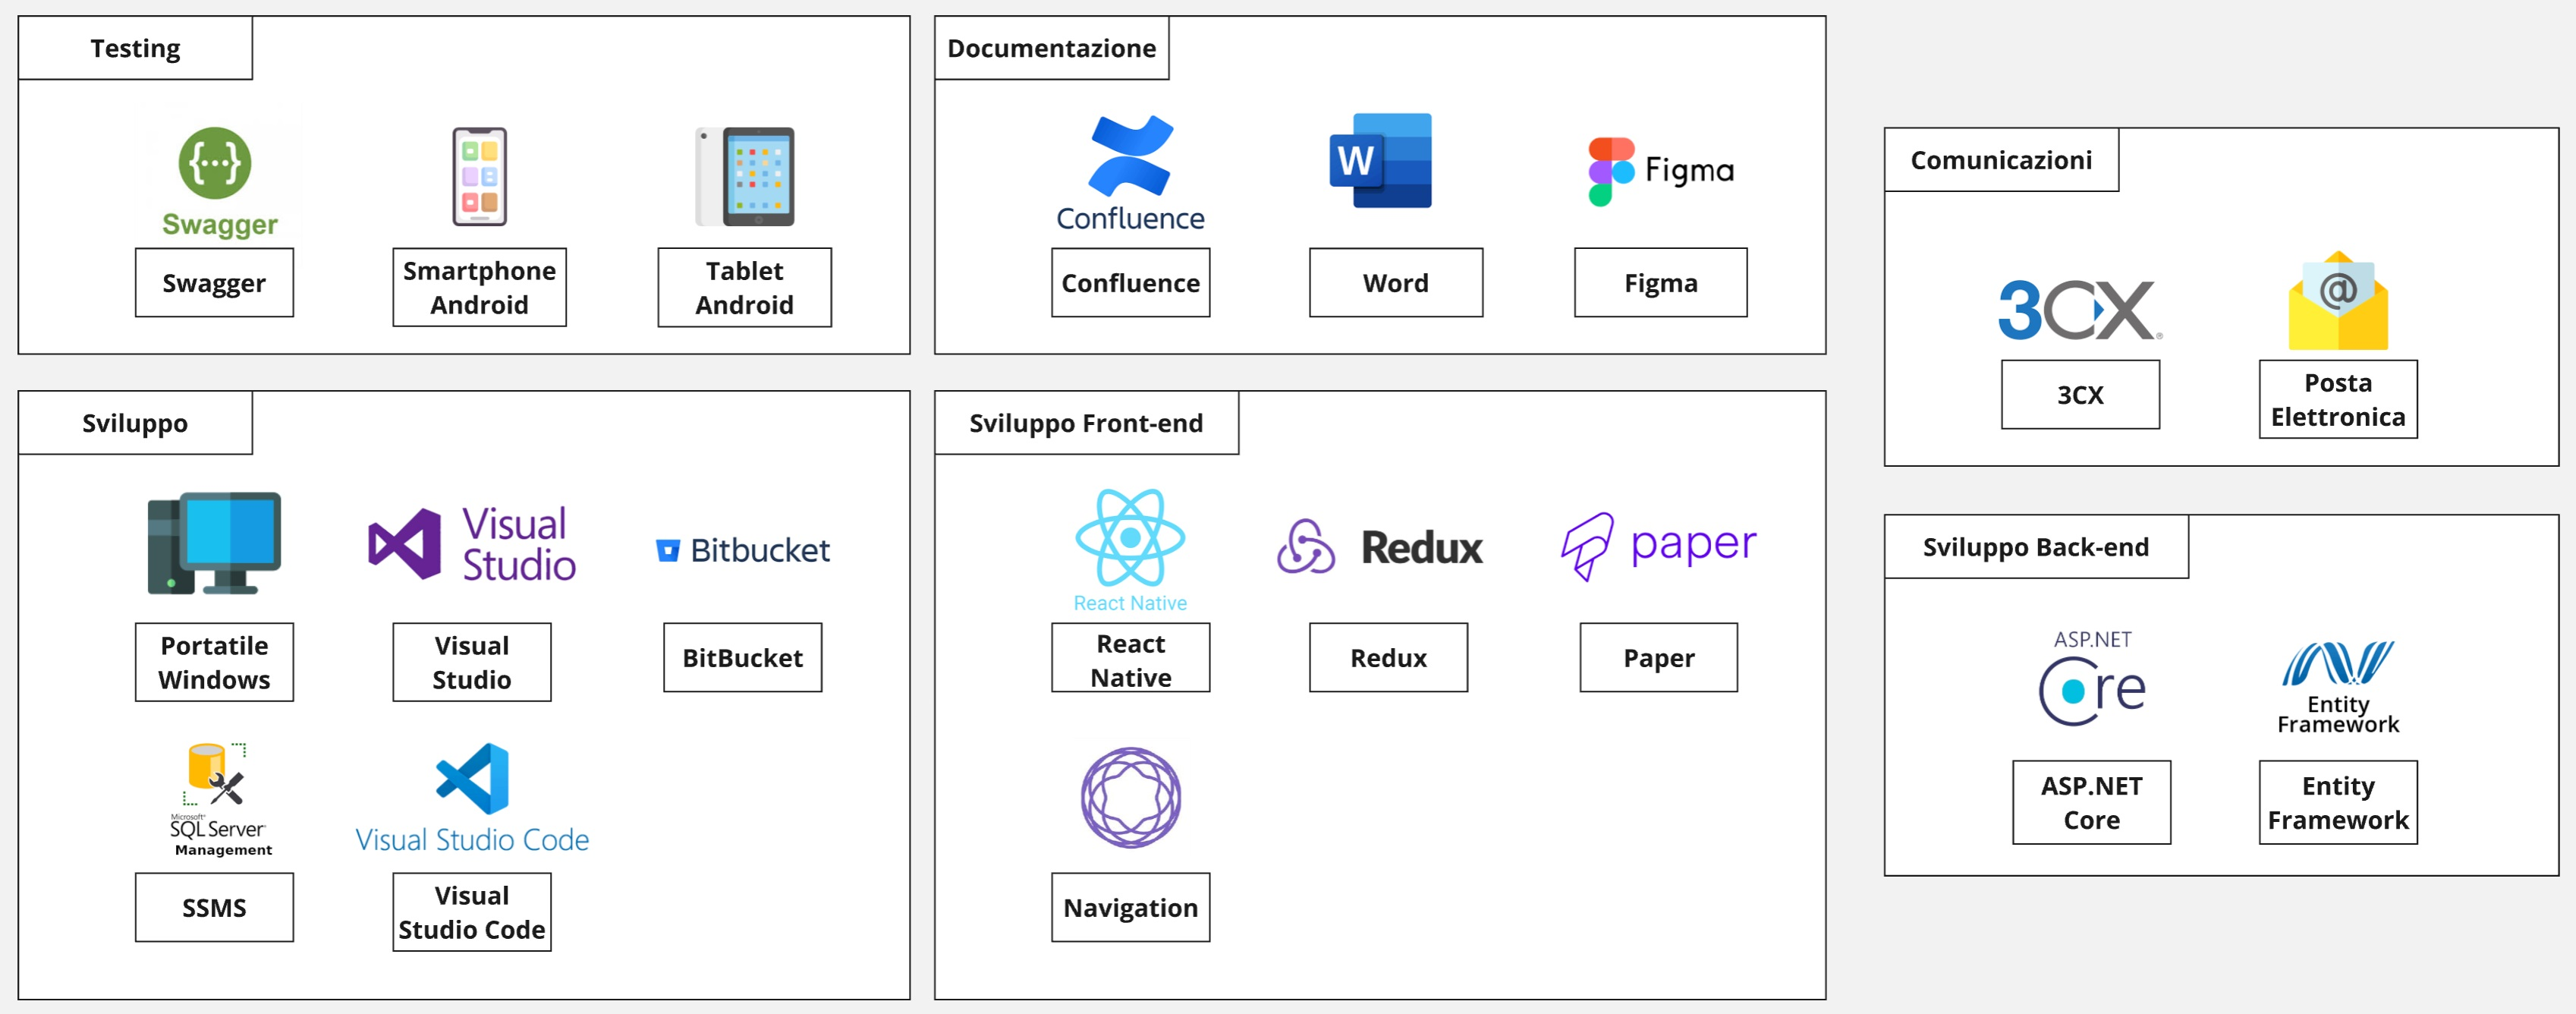
\includegraphics[alt={Tecnologie utilizzate per lo sviluppo di {\movi}}, width=\textwidth]{img/vincoli_tec.jpg}
      \caption[Tecnologie utilizzate per lo sviluppo di {\movi}]
              {Tecnologie utilizzate per lo sviluppo di {\movi}}
      \label{fig:tecnologie movi}
  \end{figure}

Le tecnologie che ho utilizzato per sviluppare il modulo agenti, come mostra la figura \ref{fig:tecnologie movi}, sono:
\begin{itemize}
      \item \textbf{Visual Studio}: per lo sviluppo delle \gls{api}. Offre numerosi strumenti per
            il \textit{debug} del codice e facilita la gestione dei pacchetti necessari.
            È particolarmente efficace per lo sviluppo in C\#, grazie alle funzioni di auto completamento
            e all'aggiornamento automatico degli \textit{import};
      \item \textbf{Visual Studio Code}: per lo sviluppo del \textit{front-end}, grazie alle numerose estensioni
            disponibili per lo sviluppo in React (come Prettier, che assicura una formattazione uniforme
            del codice);
      \item \textbf{\textit{Computer} con Windows 10}: preferito al Mac per la mia esperienza pregressa
            con Windows, evitando così l'apprendimento di un nuovo sistema operativo parallelamente alle nuove tecnologie necessarie;
      \item \textbf{\textit{Smartphone e tablet} Android}: per il \textit{testing} dell'applicazione;
      \item \textbf{BitBucket}: per conservare il codice all'interno di un \textit{branch} del progetto e usufruire delle 
            funzionalità di Git;
      \item \textbf{Confluence}: per conservare la documentazione creata;
      \item \textbf{Word}: per creare la documentazione tecnica, poiché consente di creare rapidamente e agevolmente un
            documento facilmente consultabile e modificabile;
      \item \textbf{Figma}: per creare il manuale utente. Permette una gestione dello stile più precisa e personalizzabile
            rispetto a Word, ma richiede più tempo per la creazione di un documento. Il risultato è un impatto grafico migliore,
            meno rilevante per un documento tecnico, ma apprezzabile per un documento destinato all'utente finale;
      \item \textbf{Servizio di posta elettronica}: per ricevere gli annunci aziendali;
      \item \textbf{SQL Server Management Studio (SSMS)}: per operare sul \textit{database} usato per lo sviluppo dell'
      applicazione;
      \item \textbf{Swagger}: per testare manualmente le \gls{api} e valutarne il corretto funzionamento.
\end{itemize}
Per completezza, menziono anche 3CX tra le tecnologie che mi sono state fornite. Tuttavia, non ho mai avuto necessità di utilizzarlo,
avendo avuto la possibilità di confrontarmi personalmente con gli sviluppatori e il \textit{tutor} aziendale. Inoltre, durante
il mio \textit{stage}, il \textit{meeting} mensile generale è stato annullato, impedendomi di partecipare alla video chiamata.\\
I \textit{framework} e le librerie utilizzate sono:
\begin{itemize}
      \item \textbf{React Native}: \textit{framework} che consente lo sviluppo di applicazioni Android e iOS utilizzando il
            \textit{framework} React. Include funzionalità specifiche per dispositivi \textit{mobile}, distinguendosi da
            React, principalmente utilizzato per lo sviluppo di siti \textit{web}.\\
            Permette di scrivere e mantenere un unico codice funzionante per entrambi i sistemi operativi, eliminando la necessità 
            di sviluppatori specializzati separatamente nello sviluppo Android e iOS;
      \item \textbf{React Native Paper}: libreria di componenti per le interfacce;
      \item \textbf{React Native Navigation}: libreria per la gestione della navigazione tra le \textit{view};
      \item \textbf{React Native Redux}: libreria per la gestione dello stato dell'applicazione in React Native;
      \item \textbf{ASP.NET Core}: \textit{framework open source} moderno per lo sviluppo di applicazioni connesse a \textit{internet},
            utilizzato in questo caso per lo sviluppo delle \gls{api} necessarie;
      \item \textbf{Entity Framework Core}: \gls{orm} (\textit{Object-Relational Mapping}) per .NET, un \textit{mapper} che 
            semplifica l'accesso e la gestione dei dati nel \textit{database}, permettendo di lavorare con oggetti .NET 
            invece di \textit{query} SQL.
\end{itemize}

\subsection{Vincoli temporali}\label{chap:vincoli temporali}
\begin{figure}[H]
    \centering
    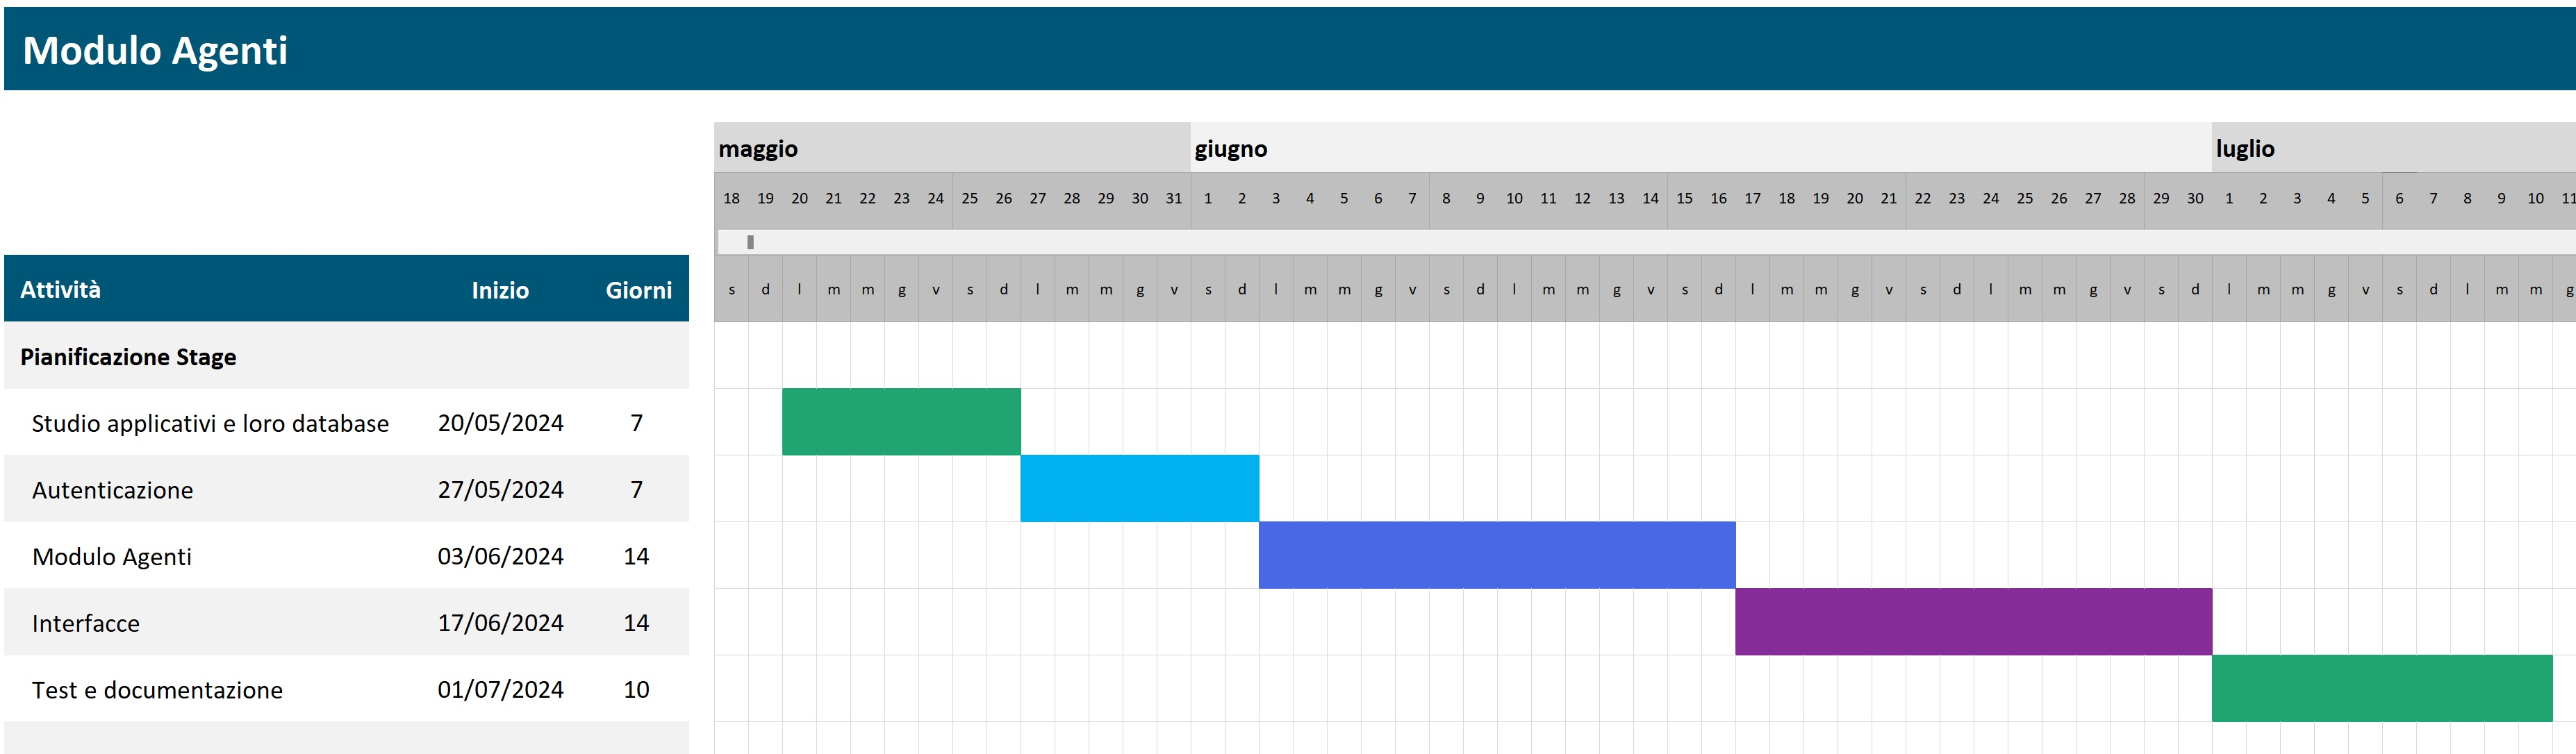
\includegraphics[alt={Pianificazione attività di stage}, width=\textwidth]{img/gantt pianificazione.jpg}
    \caption[Pianificazione attività di \textit{stage}]
            {Pianificazione attività di \textit{stage}}
    \label{fig:pianificazione stage}
\end{figure}

La figura \ref{fig:pianificazione stage} illustra la pianificazione delle mie attività di \textit{stage},
come riportata nel piano di lavoro concordato con il \textit{tutor} aziendale e approvato dal relatore.
Lo stage si divide in cinque attività principali:
\begin{enumerate}
      \item \textbf{Studio degli applicativi e del \textit{database}} (una settimana): si concentra sull'apprendimento
            delle tecnologie utilizzate e sull'analisi del codice sorgente;
      \item \textbf{Modifica della \gls{api} di autenticazione} (una settimana): l'obiettivo è modificare la \gls{api} di 
           \textit{login} per il nuovo tipo di utente agente;
      \item \textbf{Sviluppo del modulo agenti} (due settimane): prevede la creazione delle \gls{api} necessarie
            e la modifica del \textit{front-end};
      \item \textbf{Modifica delle interfacce} (due settimane): prevede la creazione dei componenti, definizione
            dello stile della UI (\textit{User Interface}) e l'ottimizzazione per \textit{tablet};
      \item \textbf{Documentazione e \textit{testing}} (dieci giorni): prevede la creazione della documentazione tecnica 
            , operativa e il \textit{testing} dell'applicazione.
\end{enumerate}